\section{Benchmark details}
\label{app:bench}

\paragraph{ARC-AGI-1.} We draw the stream from the 400 ARC-AGI-1 training tasks through the Re-ARC generators \citep{hodel2024rearc}, pinned by commit. Given a task id and a seed, the generator produces an input grid and the verifier produces its output, and we keep only the pairs that the verifier accepts, discarding any demonstration whose input equals the test input. Each demonstration request draws one more such pair. A learner cannot cache outputs, since every instance is fresh, and caching demonstrations has a price. The held-out test draws on the 400 ARC-AGI-1 evaluation tasks, which have no generators, and each of them appears once, with its original demonstrations available on request. A request returns them one at a time, two to seven of them and three or four for most tasks of the track, and nothing after them.

\paragraph{The held-out tasks are public.} The held-out test's 100 tasks come from ARC-AGI-1's public evaluation set, and 90 of them are also among ARC-AGI-2's training tasks, so a model may have met them in training. Each learner is read against itself reset, which met them as often, so what it saves there is what the stream added, not what the model brought.

\paragraph{Why the held-out test can show transfer.} ARC tasks differ in their rules but share the operations from which the rules are built. The Re-ARC generators \citep{hodel2024rearc}, from which the ARC-AGI-1 stream is drawn, implement all 400 training rules with one library of 160 primitive functions, and 53 of these primitives appear in ten or more of the generators, among them filling cells, shifting objects and filtering sets of cells (\texttt{scripts/rearc\_primitives.py}). A learner that refactors what it learns into task-specific compositions of reusable low-level primitives, and keeps the primitives, should therefore meet a held-out task with much of the machinery that the task needs already in place. Library learning has shown this on ARC, where abstractions that DreamCoder built from solved tasks let it solve progressively harder ones \citep{alford2021bidirectional}, and concept-level memory distilled from solution traces raised a language model's score over a no-memory baseline \citep{ho2025arcmemo}. None of the learners in this paper keeps such primitives. The program library stores one whole program per task, and the harnesses as shipped store prose or general advice (Appendix~\ref{app:persist}), and so we attribute the absence of transfer from notes and programs in Section~\ref{sec:results} to these learners.

\begin{table}[!h]
\centering
\footnotesize\setlength{\tabcolsep}{4pt}
\begin{tabular}{p{0.2\linewidth}p{0.36\linewidth}p{0.36\linewidth}}
\toprule
 & Kept in the harness's notes & Kept in the student's weights \\
\midrule
Taught by the student & Q: the harness as shipped \newline QE: given expert guidance, the program library's procedure and playing rules & -- \\
\addlinespace
Taught by GLM-5.3 Flash & QT: the teacher plays the stream and writes the notes, and the student plays from them \newline QTE: the teacher given the guidance \newline QETE: both given it & QDE: imitates the teacher's move in each state the student met, the teacher reading expert guidance \\
\bottomrule
\end{tabular}
\caption{The comparison on Qwen3.5-9B. Every method plays the same stream in the same harness, prime-agent, beside its wiped twin and the baselines, and the methods on each line share their teacher. The weights taught by the student alone are not shown (Appendix~\ref{app:other-weights}).}
\label{tab:design}
\end{table}

\paragraph{Task ids.} In continual learning, exposing the task id corresponds to the task-oracle setting. We expose it because recognizing that today's grid is the same kind of problem as one from last month is a separate skill from remembering how to solve it, and mixing the two would make the measurement harder to read. An input grid alone also does not determine the task, as Figure~\ref{fig:taskid} shows with pairs of training tasks whose inputs are drawn from overlapping distributions. The same grid is then a valid input to both tasks, and only the demonstrations or the id say which rule applies. A learner may key its memory on the id, as the floors, the program library and the harnesses given expert guidance do (Section~\ref{sec:baselines}). It sees the id under an alias drawn for each run. The real id would be a lookup key: on the ARC-AGI-1 track, a learner with no model that runs the Re-ARC solver named by the id, and finds each held-out input among the public evaluation files, solves every instance of the stream and the held-out tasks at no cost, and uses none of the budget without learning anything. The alias makes such a lookup cost at least one demonstration per task, since a learner can still find the task by running every solver on a pair it has bought, and so what a learner may bring to the stream is stated with the code, and a result is verified by rerunning it from its code. A task-free variant would be a different benchmark, in which the learner must first buy enough demonstrations to identify the task, and we leave it to future work.

\begin{figure}[t]
\centering
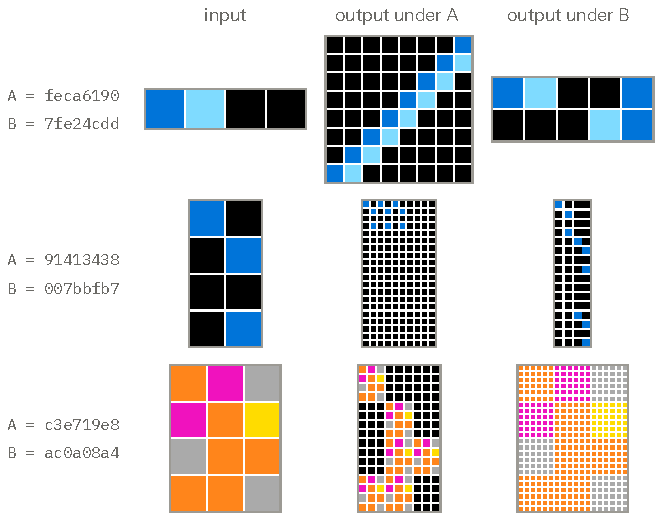
\includegraphics[width=0.66\linewidth]{figures/taskid.pdf}
\caption{An input grid does not determine its task. Each row shows one input generated for training task A, with the output of task A's rule and the output of task B's rule on the same grid. Both are valid ARC tasks, and only the demonstrations or the id say which rule applies. Top: A (\texttt{feca6190}) draws diagonal lines from each colored cell on a larger black square, and B (\texttt{7fe24cdd}) lays out the input and its three rotations as four quadrants. Middle: A (\texttt{91413438}) tiles copies of the input, one per colored cell, and B (\texttt{007bbfb7}) places the input's pattern in every tile whose cell is colored. Bottom: A (\texttt{c3e719e8}) places the whole input in every tile whose cell has the most frequent color. B (\texttt{ac0a08a4}) enlarges every cell into a block. The pairs are selected automatically: an input generated for A on which B's verifier runs and returns a different valid grid.}
\label{fig:taskid}
\end{figure}

\paragraph{Observation horizon.} As the generators produce fresh instances without end, a configuration's stream length is only the window over which we observe a learner. It places no limit on how much the learner may learn. Within a run, a checkpoint is a prefix, and it never changes when the run is carried further. Every instance is charged, so the budget used against instances is the experience curve and the budget used at a horizon is its mean (Equation~\ref{eq:score}). A system that becomes competent after fewer instances then uses less of the budget at every checkpoint, which is the kind of efficiency that \citet{chollet2019measure} asked for, and the benchmark sets no cap on data. While a learner cannot choose how many instances arrive, it can choose how many demonstrations to buy, which the score charges, and how much of its experience to train on, which we count as compute and log without scoring.

\begin{table}[t]
\centering
\small
\setlength{\tabcolsep}{4pt}
\begin{tabular}{lrrrrrrr}
\toprule
track & tasks & stream & held-out & $n_c$ & $b$ & $m$ & $a$ \\
\midrule
ARC-AGI-1 & 25  & 200       & 100 & 4  & 3      & 30      & 2   \\
\bottomrule
\end{tabular}
\caption{The ARC-AGI-1 track's configuration. Each track is its configuration, in the individual regime, at seed 0. The stream length is per user, and the held-out tasks, those of the held-out test, are the same for every user. $n_c$, $b$, $m$ and $a$ are the stream's parameters (Appendix~\ref{app:schedules}), in instances, with $\sigma = 1$ throughout. The number of users $n_u \in \{1, 2, 4\}$ is a setting of the run, not of the configuration. At four users, the stream has 200 rounds over 100 distinct tasks, with eight instances per task and four graded instances per round. Every configuration has an attempt cap of 8 and a demonstration cap of 8, one pair per request, with $c_d = 1$.}
\label{tab:configs}
\end{table}

\paragraph{Intervals and chance.} Tables report pointwise 95\% intervals from 2{,}000 paired task resamples, after averaging each instance's spend over its plays; $L$ is resampled over stream tasks. The two-test planes instead show approximate simultaneous 95\% intervals across the displayed learners, separately for each model, reasoning effort, user count, track, test and measure. For $k$ learners, we take quantiles $0.025/k$ and $1-0.025/k$ from 200{,}000 paired task resamples (Bonferroni correction). A change is detected when this interval excludes zero for share saved, or one for the solve-rate ratio. These intervals condition on the learned state: repeated tests do not measure variation across independent learning runs. Task resampling includes independent play noise, but does not capture variation shared across a whole play. Two learners differ when the pointwise 95\% interval of their paired task-by-task difference excludes zero.

\paragraph{The exposure curve.} We write $e_i$ for the exposure index of instance $i$, the number of earlier rounds in which its task appeared (in the individual regime, a round is one instance), from 0 to 7, since the tracks serve every task eight times. Over the stream records $\mathcal{S}$, we define
\begin{equation}
U(k) = \operatorname{mean}\{\, u_i : e_i = k \,\},
\label{eq:metrics}
\end{equation}
and Figure~\ref{fig:notes-weights} plots it against the visit to the task, $e_i + 1$. $U(0)$ is the acquisition cost and $U(k)$ the exposure curve. A system that replays stored demonstrations to a stateless solver moves down this curve only by the demonstrations it no longer pays for, while a system that has learned a task falls below the curve of such a replay. The curve also has a solve-rate twin, which replaces $u_i$ with $s_i$. The standard measures of average accuracy, backward transfer and forgetting \citep{lopezpaz2017gradient} assume task boundaries and a fixed test set per task, neither of which a recurring stream scored by attempts has.

\paragraph{Why a simpler reading fails.} The drop from a system's first exposures to its later ones rewards a poor start, and a stream's returning instances need not be as hard as its first ones. On the ARC-AGI-1 track at one user, the stateless floor, which cannot learn, uses more of the budget on returns than on first exposures with every model, from 3 points on Qwen3.5-9B to 16 on GPT-6 Luna at medium effort. The share learned (Equation~\ref{eq:learned}) instead pairs a learner with its own reset on the same instances. Keeping the demonstrations a task was shown is a memory like any other, and the demo-cache floor, read against the stateless floor, scores above zero. The bare model is no reference. A learner read against its own reset could score by playing worse whenever its memory is empty. On Qwen3.5-9B every reset in prime-agent does play both tests below the bare model, since the harness gives up most of their instances after replies with no readable action (Appendix~\ref{app:harness}), so Table~\ref{tab:tests-absolute} marks each such reset and gives every learner's budget beside it, and a verified result is also played bare and flagged when the reset plays below the bare model (Appendix~\ref{app:heldout}). A learner at more than one user is read against the reset at the same number of users, which met the same instances (Appendix~\ref{app:trained}).

\paragraph{Generating data at will.} \citet{chollet2019measure} also wrote that an ideal benchmark should avoid tasks for which new data can be generated at will, because performance can then be bought with data. We generate data at will deliberately, for two reasons. In the stream, every demonstration and every wrong attempt is charged, and so the measure is the feedback consumed, as he proposed, which leaves no room for the unpaid practice on the test distribution that concerned him. In the held-out test there are no generators at all, which rules out buying final skill with data where we measure transfer. The concern does survive in a weaker form, since Re-ARC covers the public training split, which any developer knows.

\paragraph{Compute.} Each record carries whatever the learner reports, as a per-instance difference in cumulative counters, including tokens, wall-clock seconds, bytes of persistent state and dollars, and, for a learner that trains on its traces, the number of instances it has trained on. The baselines report these through the accounting layer so that they do not count for themselves. We log compute without scoring it, because we do not know the exchange rate between a weight update and a hundred thousand prompt tokens, and any fixed rate would decide the comparison in advance.
